\section{后端互操作性}
在本章中,我们将了解后端互操作性,这是一种 SYCL 功能,
可以将 SYCL 增量添加到已经使用其他数据并行技术或 API 的应用程序。

我们还将了解熟悉低级 API 的专家程序员如何使用后端互操作性来“窥视幕后”并直接使用 SYCL 程序中的底层数据并行 API。 
这可以在必要时直接访问特定于 API 的功能,同时保留 SYCL 的可移植性和易用性优势。

\subsection{什么是后端互操作性?}
\begin{figure}[H]
	\centering
	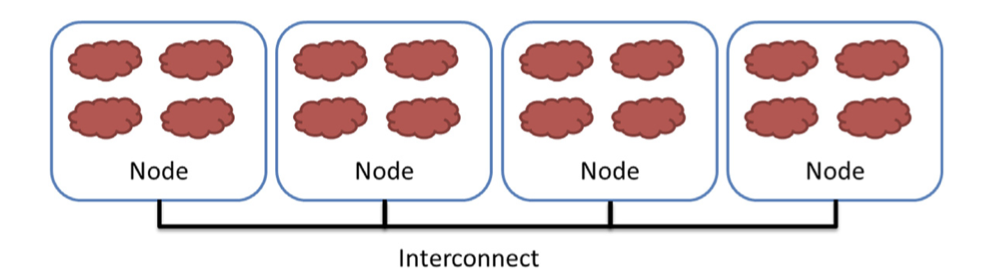
\includegraphics[width=0.9\textwidth]{figs/F20.1.png}
	\caption{\textit{SYCL 后端、平台和设备之间的关系 }}
\end{figure}

到目前为止,在本书中,我们提到了在 SYCL 设备上运行的 SYCL 程序,
但实际上,许多 SYCL 实现都基于较低级别的 API(例如 OpenCL、零级、CUDA 或其他 API)来访问系统中的并行硬件。 
当 SYCL 实现基于较低级别的 API 构建时,我们将目标 API 称为 SYCL 后端。 
图20-1显示了SYCL后端、平台和设备之间的关系。 
大多数 SYCL 实现可以同时在多个 SYCL 后端上运行 SYCL 程序,以利用系统中的所有并行硬件。

\begin{figure}[H]
	\centering
	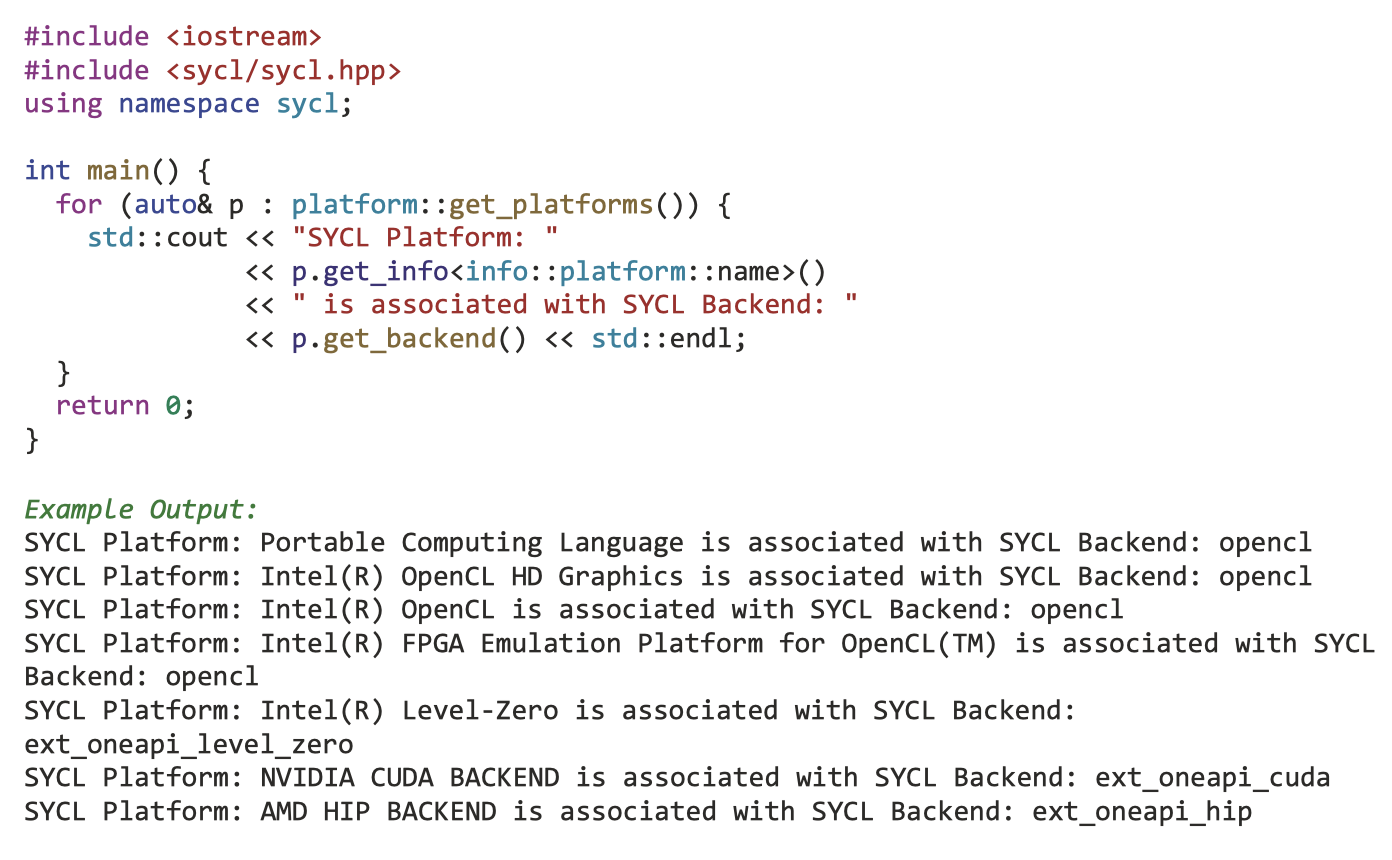
\includegraphics[width=0.9\textwidth]{figs/F20.2.png}
	\caption{\textit{查询 SYCL 平台的 SYCL 后端 }}
\end{figure}

我们可以通过先查询SYCL平台,然后查询与每个平台关联的SYCL后端来查询系统中的SYCL后端,如图20-2所示。 
该程序的输出将取决于系统中 SYCL 设备的数量和类型。 
如果不同的 SYCL 后端支持同一设备,则它可能会为每个后端枚举为 SYCL 设备。

可以查询大多数 SYCL 对象的关联后端,而不仅仅是 SYCL 平台。 
例如,我们还可以查询关联后端的 SYCL 设备、SYCL 上下文或 SYCL 队列。

后端互操作性使我们能够使用关联后端的知识来与代表关联后端的 SYCL 对象的底层本机后端对象进行交互并进行操作。

\subsection{后端互操作性何时有用?}
许多 SYCL 程序员永远不需要使用后端互操作性。 事实上,使用后端互操作性可能是不可取的; 
后端互操作性通常会导致程序变得更加复杂,因为它需要多个 SYCL 后端的多个代码路径,
或者会降低程序的可移植性,因为它将限制执行到具有单个关联后端的设备。

尽管如此,后端互操作性仍然是我们工具箱中解决某些特定问题的有用工具。 
在本节中,我们将探讨后端互操作性有用的几个常见用例。

\begin{remark}[后端互操作性就像一个内联汇编程序]
后端互操作性的一个有用心智模型是,后端互操作性之于 SYCL,就像内联汇编程序之于 C++ 主机代码一样:
后端互操作性对于学习 SYCL 或使用 SYCL 提高工作效率不是必需的,并且后端互操作性通常是不可取的,
因为它会增加复杂性或降低可移植性。尽管如此,它是我们工具箱中解决特定问题的有用工具。
\end{remark}

\subsubsection{将 SYCL 添加到现有代码库}
本书中的 SYCL 程序旨在教授特定的 SYCL 概念,因此它们故意简单明了且简短。 
相比之下,大多数现实世界的软件都是庞大而复杂的,由数千或数百万行代码组成,可能是由许多人多年来开发的。 
即使我们想这样做,完全重写大型应用程序以使用 SYCL 也可能不可行。

后端互操作性提供的主要优势之一是能够通过从该 API 的本机后端对象创建 SYCL 对象,
将 SYCL 增量添加到已使用低级 API 的现有代码库。 
例如,假设我们有一个大型 OpenCL 应用程序,它创建 OpenCL 上下文和 OpenCL 内存对象。 
后端互操作性具有 make\_context 和 make\_buffer 等模板化函数,使我们可以从这些 OpenCL 对象无缝创建 SYCL 对象。 
从 OpenCL 对象创建 SYCL 对象后,它们可以被 SYCL 队列和 SYCL Kernel使用,
就像任何其他 SYCL 对象一样,如图 20-3 所示。

\begin{figure}[H]
	\centering
	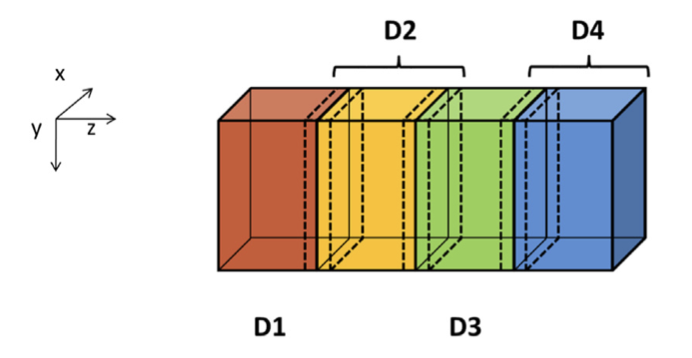
\includegraphics[width=0.9\textwidth]{figs/F20.3.png}
	\caption{\textit{从 OpenCL 对象创建 SYCL 对象 }}
\end{figure}

SYCL 2020 规范仅定义了与 OpenCL 后端的互操作性,但 SYCL 实现可以通过扩展提供与其他后端的互操作性。 
图 20-4 显示了如何使用 sycl\_ext\_oneapi\_backend\_level\_zero 扩展从零级对象创建 SYCL 对象。

\begin{figure}[H]
	\centering
	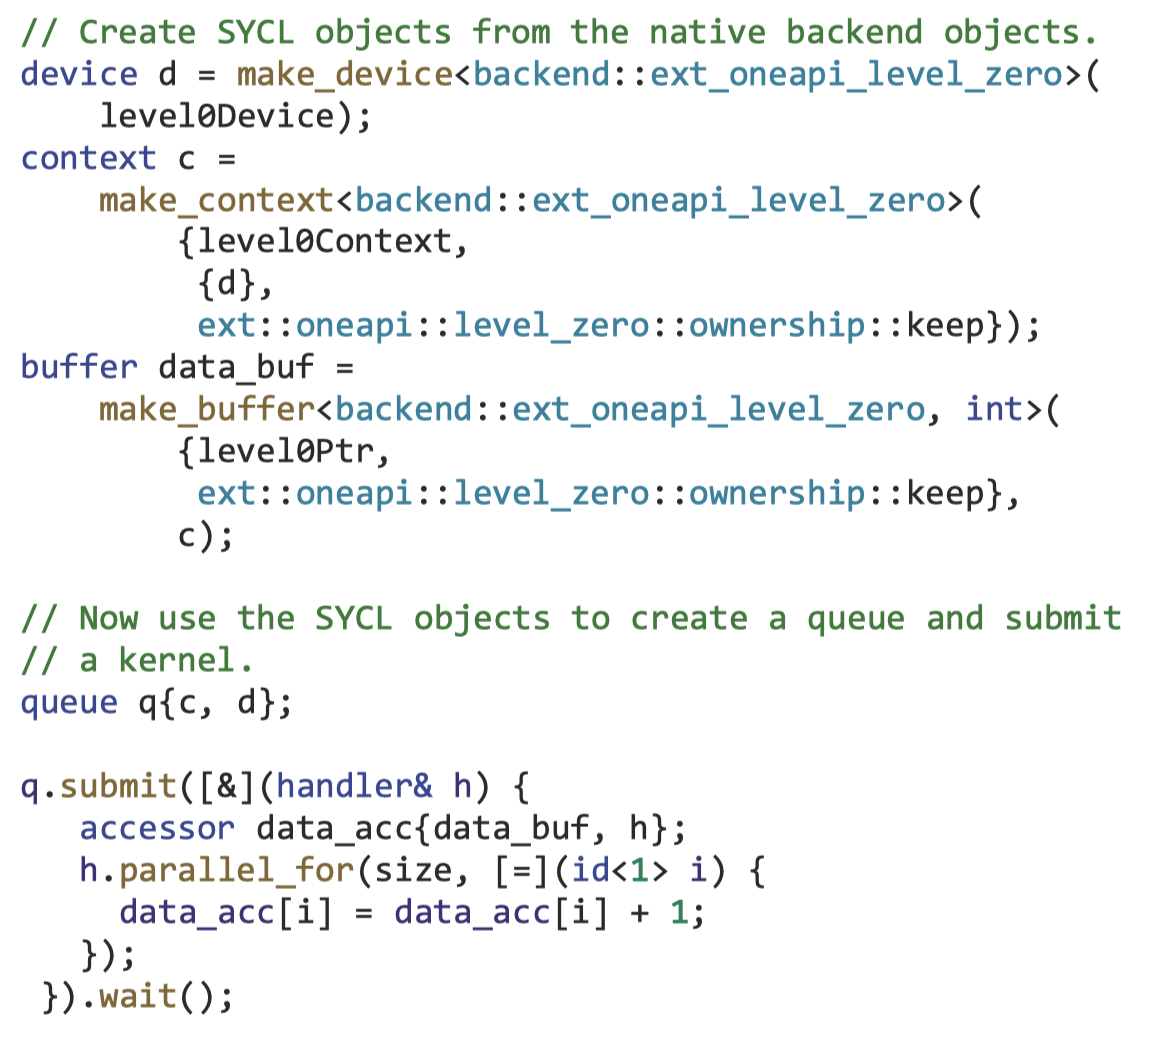
\includegraphics[width=0.9\textwidth]{figs/F20.4.png}
	\caption{\textit{从 Level Zero 对象创建 SYCL 对象 }}
\end{figure}

请注意,对于零级后端,创建 SYCL 对象时传递的参数略有不同。 
对于任何受支持的后端互操作性来说,这通常都是正确的,因为每个后端可能需要不同的信息来正确创建 SYCL 对象。 
否则,相同的 make\_device、make\_context 和 make\_buffer 函数将用于 OpenCL 和零级后端互操作性。

另请注意,每个后端对所有权的处理方式不同。 
对于 OpenCL 后端,SYCL 实现使用 OpenCL 提供的引用计数来管理本机后端对象的生命周期。 
对于零级后端,必须明确告知 SYCL 实现是否应该获取本机后端对象的所有权,或者我们的应用程序是否将保留所有权。 
如果 SYCL 实现拥有本机后端对象的所有权,则当 SYCL 对象被销毁时,本机后端对象也将被销毁; 
否则,我们的应用程序负责直接释放本机后端对象。

\subsubsection{将现有库与 SYCL 结合使用}
后端互操作性还可用于从 SYCL 对象中提取本机后端对象。 
这对于在我们的 SYCL 应用程序中使用现有的低级库或其他辅助函数非常有用。 
有两种方法可以执行此操作:第一种方法使用 get\_native 自由函数从 SYCL 对象获取本机后端对象。 
第二个使用 host\_task 和 interop\_handle 从 SYCL 运行时调度的代码中的 SYCL 对象获取本机后端对象。

\paragraph{使用自由函数获取后端对象}

\begin{figure}[H]
	\centering
	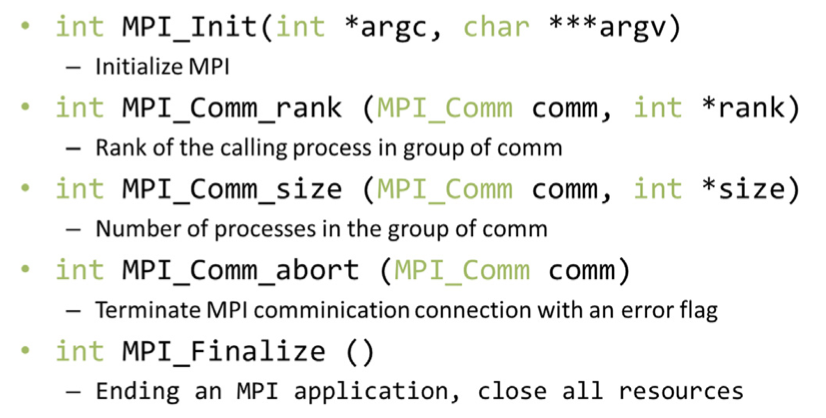
\includegraphics[width=0.9\textwidth]{figs/F20.5.png}
	\caption{\textit{使用 get\_native 自由函数从 SYCL 对象中提取 OpenCL 对象 }}
\end{figure}

例如,假设我们有一个优化的 OpenCL 库,我们希望将其与 SYCL 应用程序一起使用。 
我们可以调用后端互操作性 get\_native 函数从 SYCL 对象中获取本机 OpenCL 对象,然后可以将其与 OpenCL 库一起使用。 
为简单起见,图 20-5 中的代码仅执行查询并使用本机 OpenCL 对象分配一些内存,
但它们也可以用于执行更复杂的操作,例如创建命令队列、编译程序和执行Kernel。

\begin{figure}[H]
	\centering
	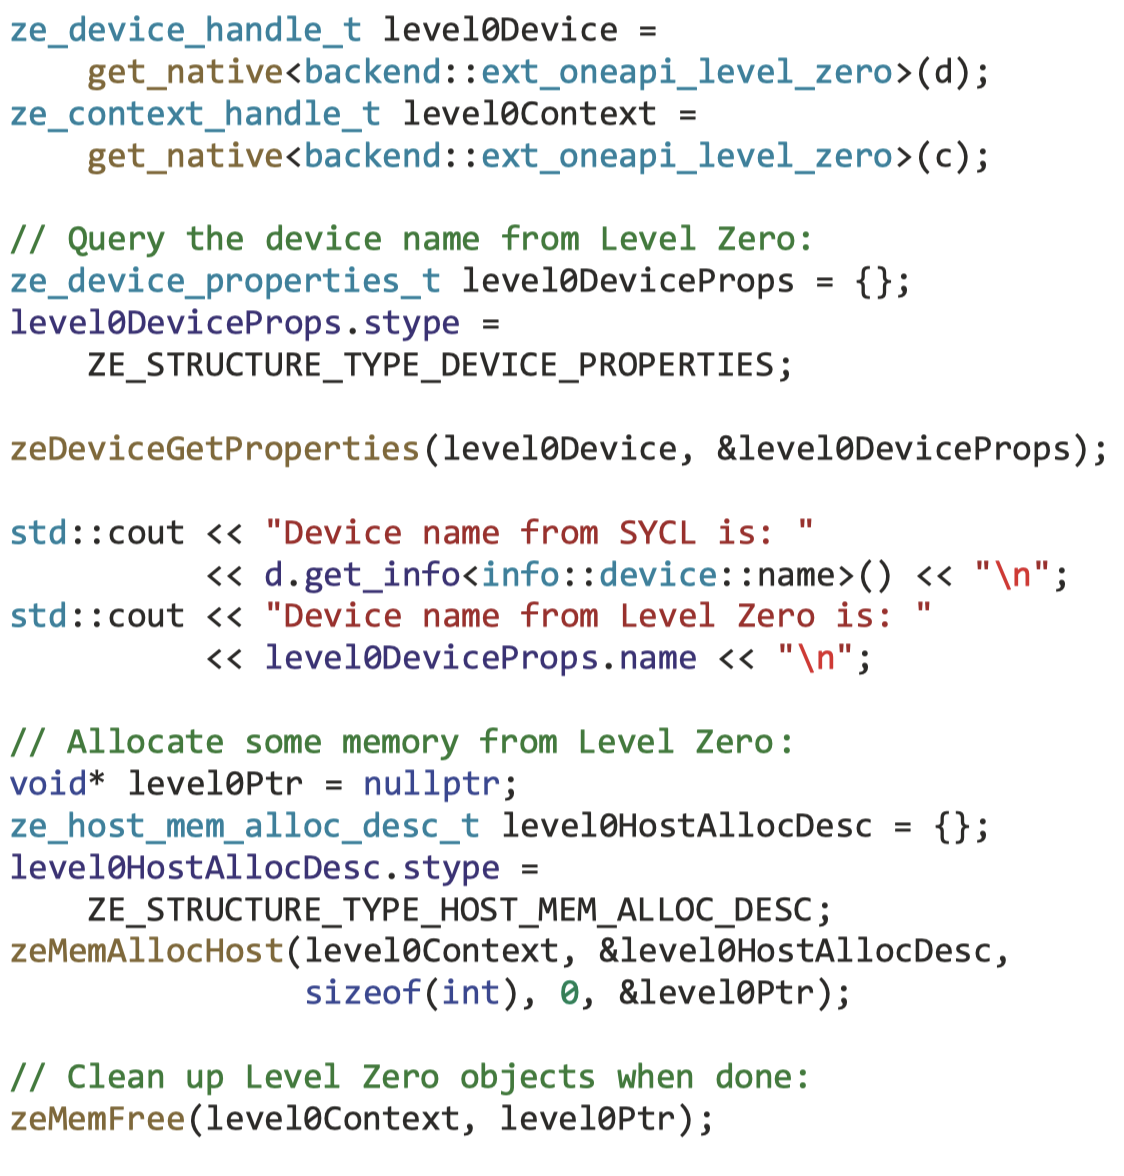
\includegraphics[width=0.9\textwidth]{figs/F20.6.png}
	\caption{\textit{使用 get\_native 自由函数从 SYCL 对象中提取 Level Zero 对象 }}
\end{figure}

作为 sycl\_ext\_oneapi\_backend\_level\_zero 扩展的一部分,
还为零级后端添加了相同的 get\_native 函数,如图 20-6 所示。

\paragraph{通过互操作句柄获取后端对象}

使用 get\_native 自由函数是获取直接使用后端 API 的大段代码的后端特定对象的有效方法。 
但在许多情况下,我们只想使用后端 API 在 SYCL 任务图中执行特定操作。 
在这些情况下,我们可以使用带有特殊 interop\_handle 参数的 SYCL host\_task 来执行特定于后端的操作。 
interop\_handle 表示调用主机任务时 SYCL 运行时的状态,
并提供对表示 SYCL 队列、设备、上下文以及为主机任务捕获的任何缓冲区的本机后端对象的访问。

\begin{figure}[H]
	\centering
	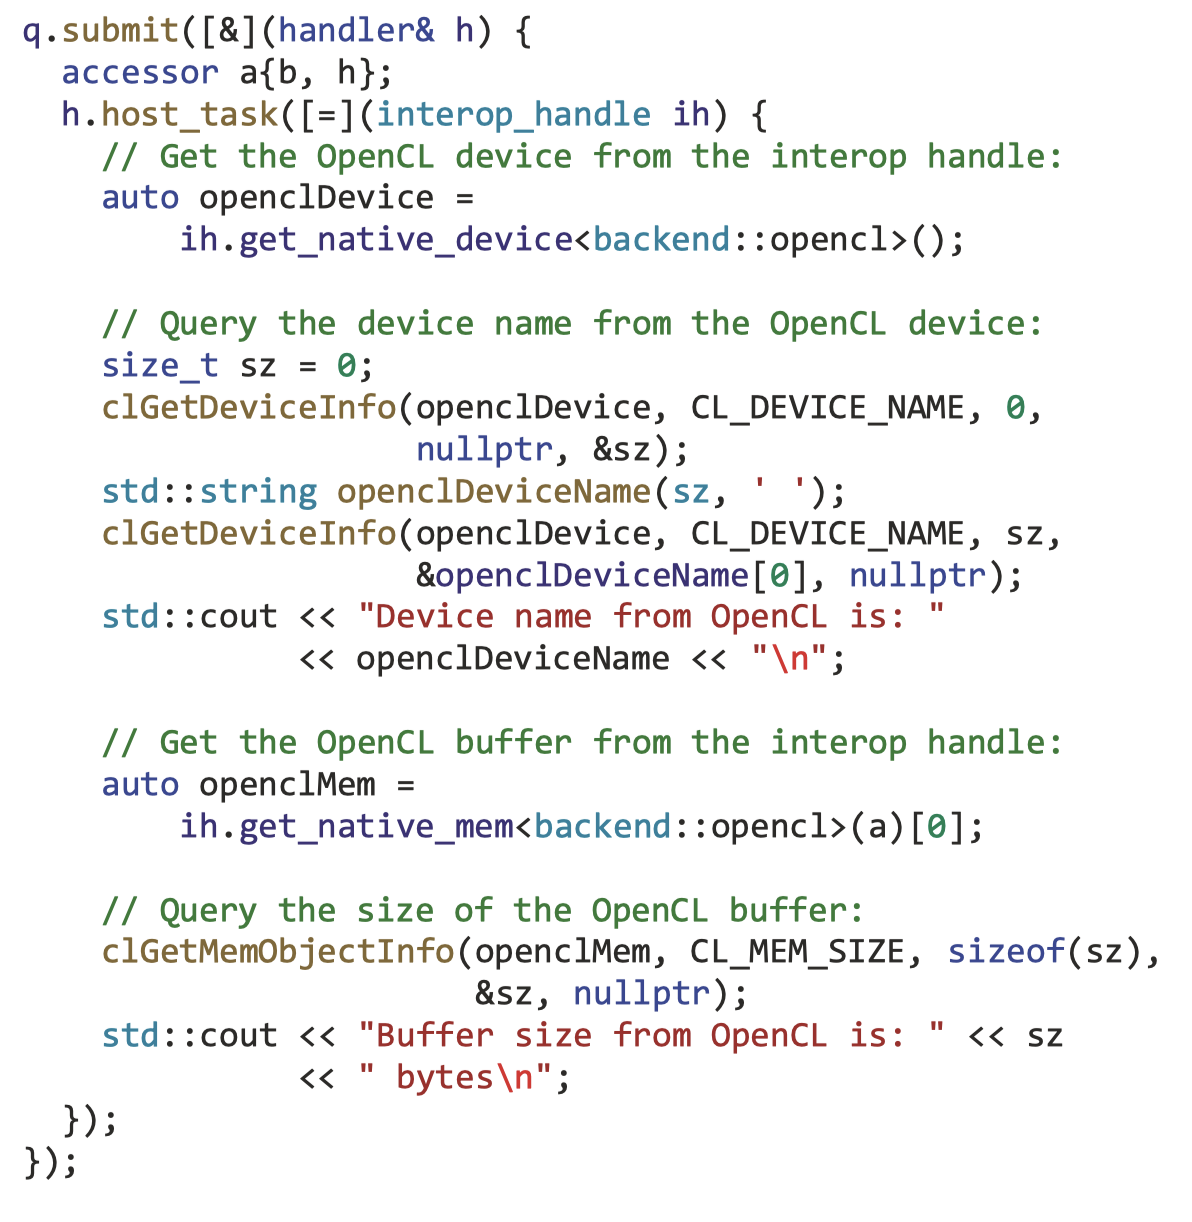
\includegraphics[width=0.9\textwidth]{figs/F20.7.png}
	\caption{\textit{使用interop\_handle从 SYCL 对象中提取 OpenCL 对象 }}
\end{figure}

图 20-7 显示了如何使用 interop\_handle 从 SYCL 运行时调度的 host\_task 获取本机 OpenCL 对象。 
为简单起见,此示例也仅使用本机 OpenCL 对象执行一些查询,
但实际应用程序代码通常会使用本机 OpenCL 对象对Kernel进行排队或调用库。 
由于这些操作是从主机任务执行的,因此它们将与 SYCL 队列中的任何其他操作一起正确调度。

请注意,当我们的访问器获取本机 OpenCL 对象时,
interop\_handle 的 get\_native\_mem 成员函数返回 cl\_mem 内存对象的向量。 
这是 SYCL 2020 规范中的要求,其中 interop\_handle 的成员函数的返回类型必须与 get\_native 自由函数匹配,
但对于 interop\_handle 用法,我们可以简单地使用向量的第一个元素。

\begin{figure}[H]
	\centering
	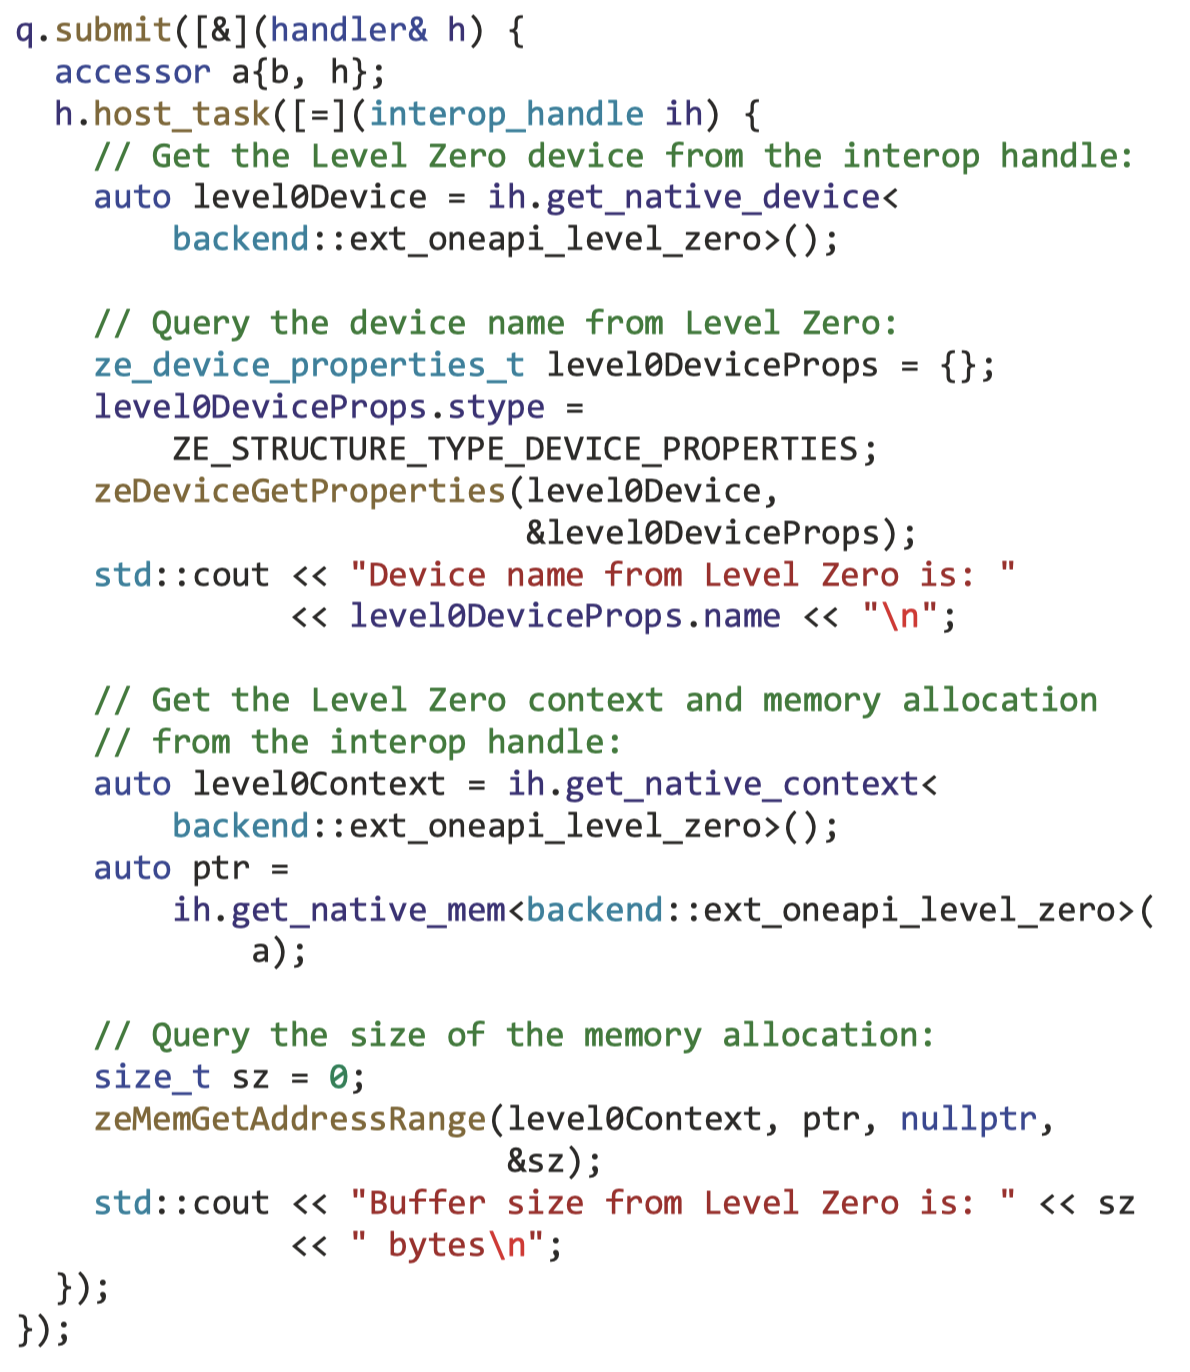
\includegraphics[width=0.9\textwidth]{figs/F20.8.png}
	\caption{\textit{使用interop\_handle从 SYCL 对象中提取 OpenCL 对象 }}
\end{figure}

与 get\_native 免费函数一样,也可以通过扩展为其他 SYCL 后端提供类似的功能。 
图 20-8 显示了如何使用 sycl\_ext\_oneapi\_backend\_level\_zero 扩展对零级后端执行类似的操作。

\subsection{使用Kernel的后端互操作性}
本节介绍如何使用后端互操作性来编译Kernel和操作Kernel包。 
这是 SYCL 2020 中经过重大重新设计的区域,以提高稳健性并增加支持不同 SYCL 后端所需的灵活性。

早期版本的 SYCL 支持两种Kernel互操作机制。 第一种机制允许从 API 定义的句柄创建Kernel。 
第二个支持从 API 定义的源或中间表示(例如 OpenCL C 源或 SPIR-V 中间表示)创建Kernel。 
这两种机制在 SYCL 2020 中仍然存在,尽管这两种机制的语法已更新并且现在使用后端互操作性。

\subsubsection{与 API 定义的Kernel对象的互操作性}
通过这种形式的互操作性,Kernel对象本身是使用低级 API 创建的,然后使用后端互操作性导入到 SYCL 中。 
图 20-9 中的代码显示了如何从 SYCL 上下文获取 OpenCL 上下文,
如何使用此 OpenCL 上下文创建 OpenCL Kernel,以及如何从 OpenCL Kernel对象创建和使用 SYCL Kernel。

\begin{figure}[H]
	\centering
	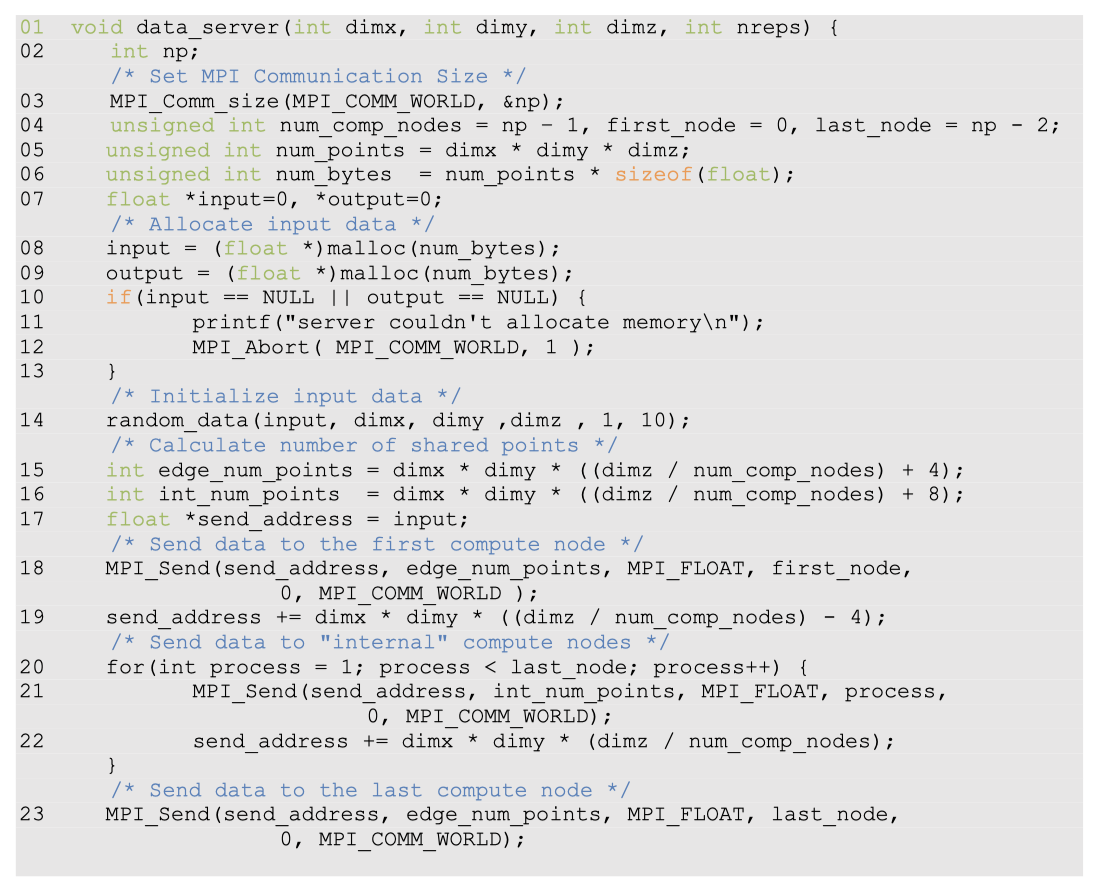
\includegraphics[width=0.9\textwidth]{figs/F20.9.png}
	\caption{\textit{从 OpenCL Kernel对象创建的Kernel }}
\end{figure}

由于 SYCL 编译器无法直接查看使用低级 API 创建的 SYCL Kernel,
因此必须使用 set\_arg() 或 set\_args() 接口显式传递任何Kernel参数。 
此外,SYCL 运行时和低级 API Kernel必须就将对象作为Kernel参数传递的约定达成一致。 
该约定应被描述为后端互操作性规范的一部分。 在此示例中,访问器 data\_acc 作为全局指针Kernel参数数据传递。

\begin{remark}
	SYCL 2020 标准将 set\_arg() 和 set\_args() 接口的精确语义留给每个 SYCL 后端规范定义。
	这允许灵活性,但这是我们编写的使用后端互操作性的代码可能特定于我们目标的后端的另一种方式。
\end{remark}

\subsubsection{与非 SYCL 源语言的互操作性}
通过这种形式的互操作性,Kernel的内容被描述为源代码或未由 SYCL 定义的中间表示形式。 
这种形式的互操作性允许重用以其他源语言编写的Kernel库或使用以中间表示形式生成代码的特定于域的语言 (DSL)。

SYCL 的早期版本包含诸如 build\_with\_source 之类的函数,
可直接从 API 定义的源语言创建 SYCL 程序,但此功能在 SYCL 2020 中被删除。
当后端直接支持 API 定义的源语言时,例如使用的 OpenCL C Kernel 对于图20-9中的OpenCL后端,
这种删除不是问题,但是如果后端不直接支持特定的源语言,我们该怎么办?

\begin{figure}[H]
	\centering
	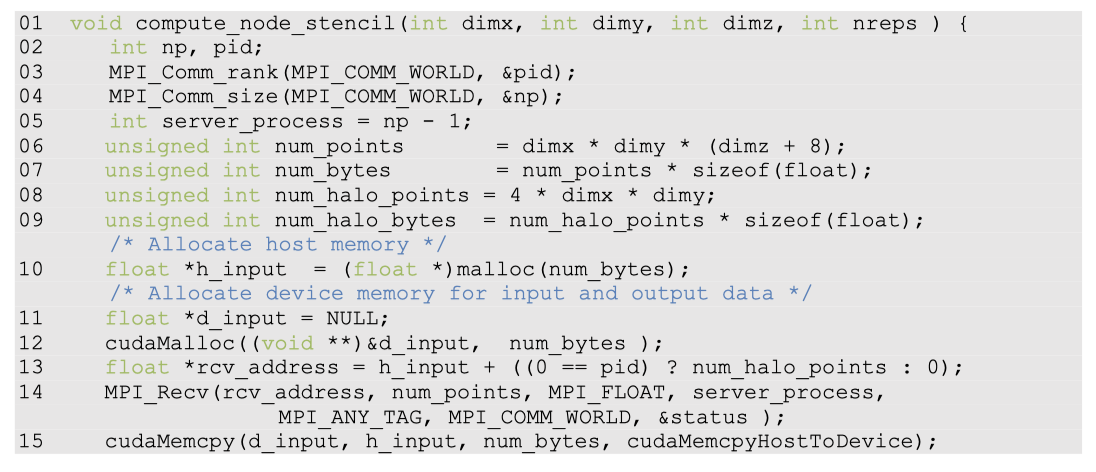
\includegraphics[width=0.9\textwidth]{figs/F20.10.png}
	\caption{\textit{使用 SPIR-V 和在线编译器创建的Kernel }}
\end{figure}

一些SYCL实现可以提供显式在线编译器来从后端不能直接使用的源语言编译为后端支持的不同格式。 
图 20-10 显示了如何使用实验性 sycl\_ext\_intel\_online\_compiler 扩展
从零级后端不支持的 OpenCL C 源代码编译为零级后端支持的 SPIR-V 中间表示形式。 
使用这种方法,Kernel可以被任何后端使用,只要它可以被在线编译器编译成后端支持的格式。

\begin{remark}[注意,实验性扩展!]
sycl\_ext\_intel\_online\_compiler扩展是一个实验性扩展,因此可能会更改或删除!
我们之所以将它包含在本书中,是因为它提供了一种实现与以前的 SYCL build\_with\_source 函数类似的功能的方法,
并且因为它是演示特定领域语言如何与 SYCL 后端交互以执行Kernel的便捷方法。
\end{remark}

在此示例中,Kernel源字符串在与 SYCL 主机 API 调用相同的文件中表示为 C++ 原始字符串文字,
但不要求是这种情况,并且某些应用程序可能会从文件中读取Kernel源字符串 甚至及时生成它。

和以前一样,由于 SYCL 编译器无法查看以 API 定义的源语言编写的 SYCL Kernel,
因此必须使用 set\_arg() 或 set\_args() 接口显式传递任何Kernel参数。

\subsection{后端互操作性提示和技巧}
本节介绍有效使用后端互操作性的实用提示和技巧。

\subsubsection{为特定后端选择设备}
正确使用后端互操作性的第一个要求是选择与所需 SYCL 后端关联的 SYCL 设备。 
有几种方法可以实现这一点。

第一个是通过在对每个设备评分时查询关联的后端,将所需的 SYCL 后端集成到现有的自定义设备选择逻辑中。 
如果我们的应用程序已经在使用自定义设备选择逻辑,那么这应该是一个简单的添加。 
该机制也是可移植的,因为它仅使用标准 SYCL 查询。

\begin{figure}[H]
	\centering
	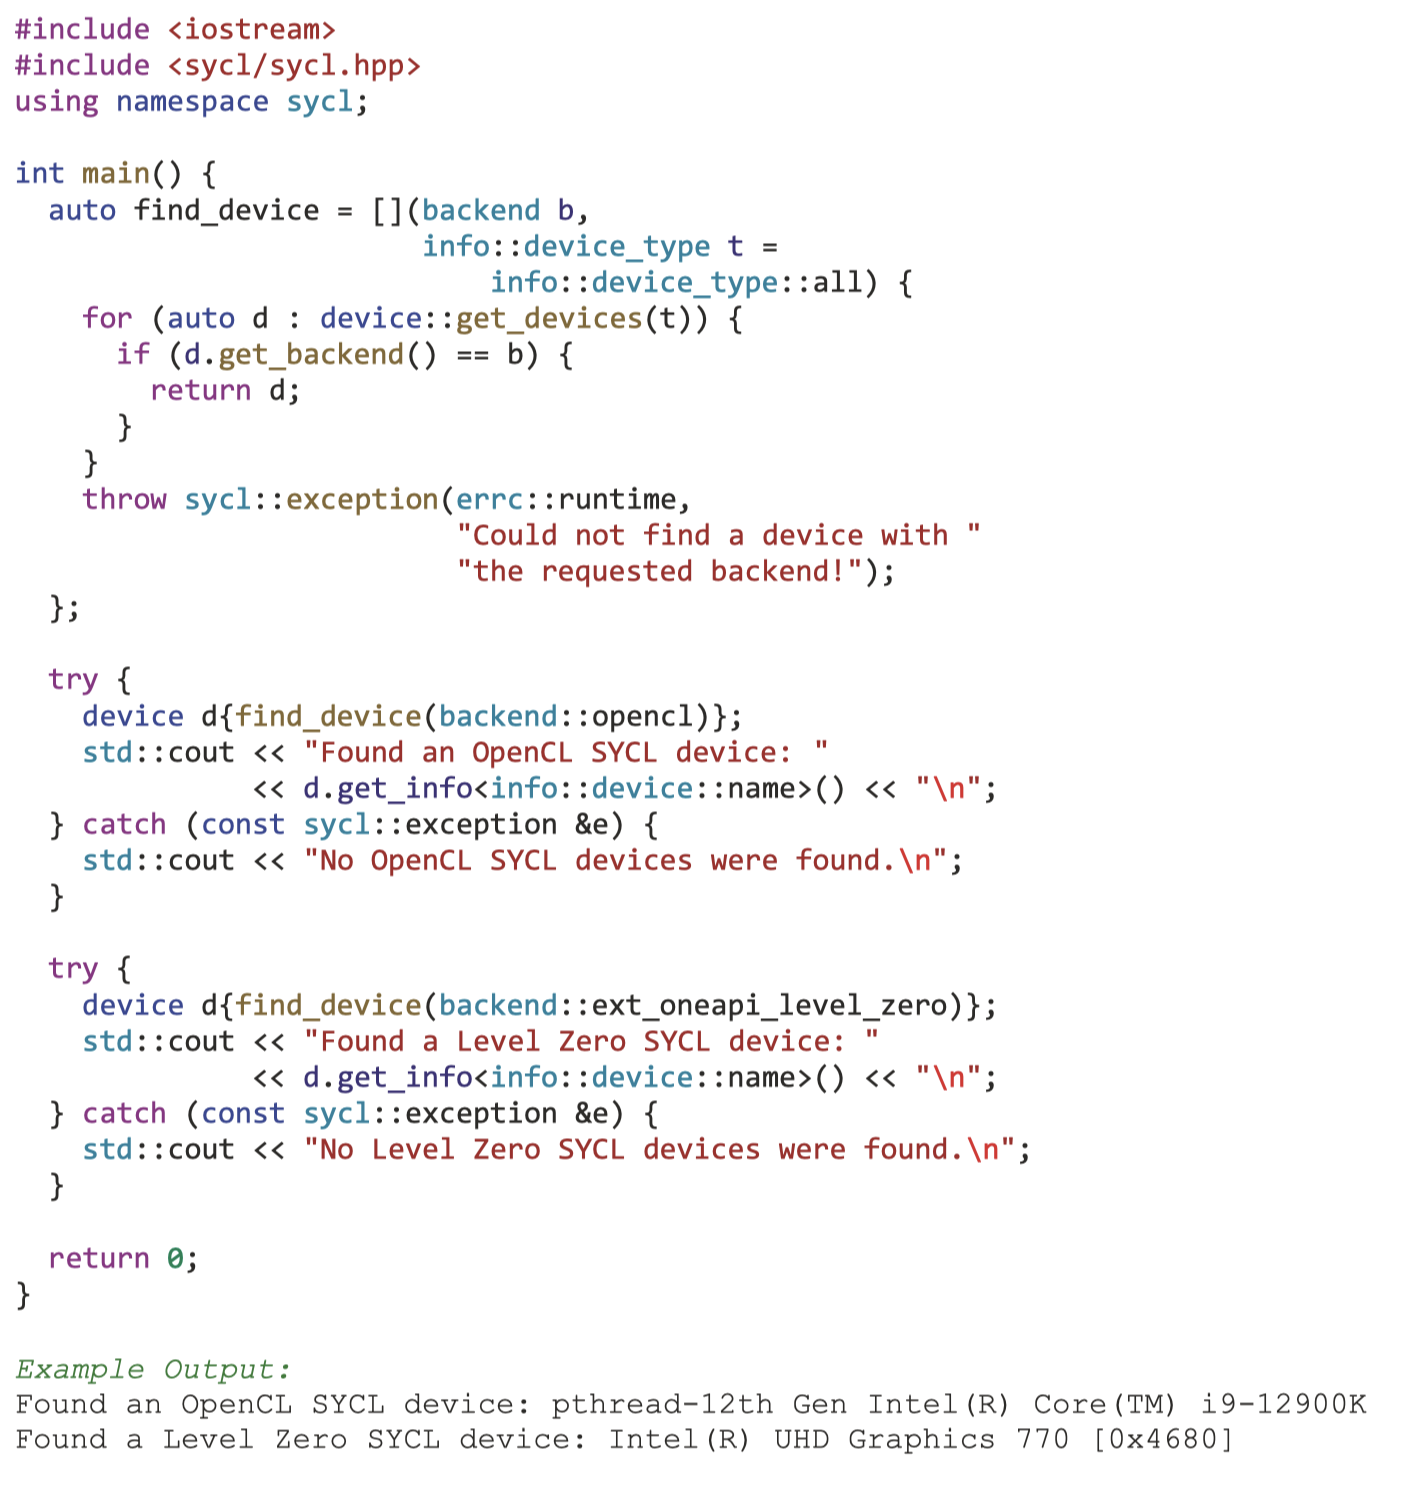
\includegraphics[width=0.9\textwidth]{figs/F20.11.png}
	\caption{\textit{查找具有特定后端的 SYCL 设备 }}
\end{figure}

对于尚未使用自定义设备选择逻辑的应用程序,我们可以编写一个简短的 C++ lambda 表达式来迭代所有设备,
以查找具有所请求后端的设备,如图 20-11 所示。 
由于此版本的 find\_device 不请求特定的设备类型,因此它实际上是标准 default\_selector\_v 的替代品。

最后,为了快速原型化,一些 SYCL 实现可以使用外部机制(例如环境变量)来影响它们枚举的 SYCL 设备。 
例如,DPC++ SYCL 运行时可以使用 ONEAPI\_DEVICE\_SELECTOR 环境变量
将枚举设备限制为特定设备类型或关联的设备后端(请参阅第 13 章)。 
对于生产代码来说,这不是一个理想的解决方案,因为它需要外部配置,
但对于原型代码来说,它是一种有用的机制,可以确保应用程序使用来自特定后端的特定设备。

\subsubsection{小心上下文!}
回想一下第 6 章和第 13 章,许多 SYCL 对象(例如Kernel和 USM 分配)如果是在不同的 SYCL 上下文中创建的,
通常无法通过 SYCL 上下文访问。 使用后端互操作性时仍然如此; 
因此,使用后端 API 创建的特定于后端的上下文通常无法访问在不同 SYCL 上下文中创建的对象(反之亦然),
即使 SYCL 上下文与同一后端关联也是如此。

为了在 SYCL 和后端之间安全地共享对象,我们应该始终使用 make\_context 从本机后端上下文创建 SYCL 上下文,
或者应该使用 get\_native 从 SYCL 上下文获取本机后端上下文。

\begin{remark}
	始终从本机后端上下文创建 SYCL 上下文或从 SYCL 上下文获取本机后端上下文,以便在 SYCL 和后端之间安全地共享对象!
\end{remark}

\subsubsection{访问低级 API 特性}
有时,尖端功能会先在低级 API 中提供,然后再在 SYCL 中提供,甚至作为 SYCL 扩展。 
有些功能甚至可能是特定于后端或特定于设备的,以至于它们永远不会通过 SYCL 公开。 
例如,某些本机后端 API 可以提供对具有特定属性的队列或特定加速器硬件的独特Kernel指令的访问。 
尽管我们希望并期望这些情况很少见,但当这些类型的功能存在时,我们仍然可以使用后端互操作性来访问它们。

\subsubsection{对其他后端的支持}
本章中的示例演示了后端与 OpenCL 和零级后端的互操作性,
但 SYCL 是一个不断发展的生态系统,SYCL 实现定期添加对其他后端和设备的支持。 
例如,支持 CUDA 和 HIP 后端的多个 SYCL 实现已经对与这些后端的互操作性提供了一些支持。 
检查 SYCL 实现的文档,以确定支持哪些 SYCL 后端以及它们是否支持后端互操作性!

\subsection{总结}
在本章中,我们了解了每个 SYCL 对象如何与底层 SYCL 后端关联以及如何查询系统中的 SYCL 后端。 
我们描述了后端互操作性如何为我们的 SYCL 应用程序提供直接与底层后端 API 交互的机制。 
我们讨论了这如何使我们能够将 SYCL 增量添加到直接使用后端 API 的应用程序,
或重用专门为后端 API 编写的库或实用程序函数。 
我们还讨论了后端互操作性如何通过限制应用程序将在哪些 SYCL 设备上运行来降低应用程序的可移植性。

我们专门探讨了Kernel的后端互操作性如何在 SYCL 2020 中提供早期版本 SYCL 中存在的类似功能。 
我们研究了在线编译器扩展如何启用Kernel的某些源语言,即使某些 SYCL 后端不能直接理解它们。

最后,我们回顾了在程序中有效使用后端互操作性的实用提示和技巧,
例如如何为特定 SYCL 后端选择 SYCL 设备、如何为后端互操作性设置 SYCL 上下文以及后端互操作性如何提供对 功能,
即使它们尚未添加到 SYCL 中。